% XCircuit output "config6.tex" for LaTeX input from config6.ps
\def\putbox#1#2#3#4{\makebox[0in][l]{\makebox[#1][l]{}\raisebox{\baselineskip}[0in][0in]{\raisebox{#2}[0in][0in]{\scalebox{#3}{#4}}}}}
\def\rightbox#1{\makebox[0in][r]{#1}}
\def\centbox#1{\makebox[0in]{#1}}
\def\topbox#1{\raisebox{-0.60\baselineskip}[0in][0in]{#1}}
\def\midbox#1{\raisebox{-0.20\baselineskip}[0in][0in]{#1}}
   \scalebox{1}{
   \normalsize
   \parbox{6.91667in}{
   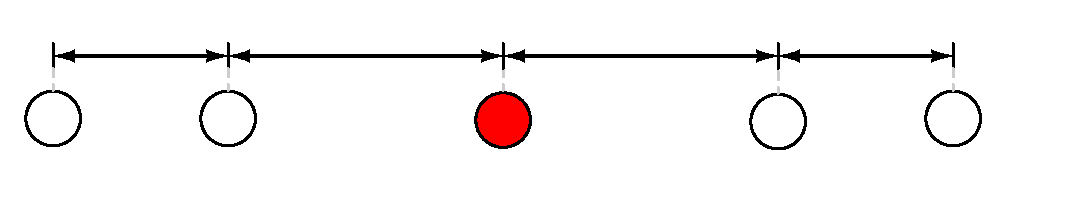
\includegraphics[scale=1]{config6}\\
   % translate x=548 y=272 scale 0.38
   \putbox{3.2in}{0.08in}{1.20}{$\lambda$}%
   \putbox{4.99in}{0.06in}{1.20}{$\lambda/2$}%
   \putbox{2.04in}{0.97in}{1.20}{$\lambda/2$}%
   \putbox{1.22in}{0.08in}{1.20}{$\lambda/2$}%
   \putbox{6.1in}{0.08in}{1.20}{$\lambda/4$}%
   \putbox{0.66in}{0.97in}{1.20}{$\lambda/4$}%
   \putbox{5.5in}{0.95in}{1.20}{$\lambda/4$}%
   \putbox{0.06in}{0.08in}{1.20}{$\lambda/4$}%
   \putbox{4in}{0.95in}{1.20}{$\lambda/2$}%
   } % close 'parbox'
   } % close 'scalebox'
   \vspace{-\baselineskip} % this is not necessary, but looks better
